\documentclass[twoside]{book}

% Packages required by doxygen
\usepackage{fixltx2e}
\usepackage{calc}
\usepackage{doxygen}
\usepackage[export]{adjustbox} % also loads graphicx
\usepackage{graphicx}
\usepackage[utf8]{inputenc}
\usepackage{makeidx}
\usepackage{multicol}
\usepackage{multirow}
\PassOptionsToPackage{warn}{textcomp}
\usepackage{textcomp}
\usepackage[nointegrals]{wasysym}
\usepackage[table]{xcolor}

% Font selection
\usepackage[T1]{fontenc}
\usepackage[scaled=.90]{helvet}
\usepackage{courier}
\usepackage{amssymb}
\usepackage{sectsty}
\renewcommand{\familydefault}{\sfdefault}
\allsectionsfont{%
  \fontseries{bc}\selectfont%
  \color{darkgray}%
}
\renewcommand{\DoxyLabelFont}{%
  \fontseries{bc}\selectfont%
  \color{darkgray}%
}
\newcommand{\+}{\discretionary{\mbox{\scriptsize$\hookleftarrow$}}{}{}}

% Page & text layout
\usepackage{geometry}
\geometry{%
  a4paper,%
  top=2.5cm,%
  bottom=2.5cm,%
  left=2.5cm,%
  right=2.5cm%
}
\tolerance=750
\hfuzz=15pt
\hbadness=750
\setlength{\emergencystretch}{15pt}
\setlength{\parindent}{0cm}
\setlength{\parskip}{3ex plus 2ex minus 2ex}
\makeatletter
\renewcommand{\paragraph}{%
  \@startsection{paragraph}{4}{0ex}{-1.0ex}{1.0ex}{%
    \normalfont\normalsize\bfseries\SS@parafont%
  }%
}
\renewcommand{\subparagraph}{%
  \@startsection{subparagraph}{5}{0ex}{-1.0ex}{1.0ex}{%
    \normalfont\normalsize\bfseries\SS@subparafont%
  }%
}
\makeatother

% Headers & footers
\usepackage{fancyhdr}
\pagestyle{fancyplain}
\fancyhead[LE]{\fancyplain{}{\bfseries\thepage}}
\fancyhead[CE]{\fancyplain{}{}}
\fancyhead[RE]{\fancyplain{}{\bfseries\leftmark}}
\fancyhead[LO]{\fancyplain{}{\bfseries\rightmark}}
\fancyhead[CO]{\fancyplain{}{}}
\fancyhead[RO]{\fancyplain{}{\bfseries\thepage}}
\fancyfoot[LE]{\fancyplain{}{}}
\fancyfoot[CE]{\fancyplain{}{}}
\fancyfoot[RE]{\fancyplain{}{\bfseries\scriptsize Generated by Doxygen }}
\fancyfoot[LO]{\fancyplain{}{\bfseries\scriptsize Generated by Doxygen }}
\fancyfoot[CO]{\fancyplain{}{}}
\fancyfoot[RO]{\fancyplain{}{}}
\renewcommand{\footrulewidth}{0.4pt}
\renewcommand{\chaptermark}[1]{%
  \markboth{#1}{}%
}
\renewcommand{\sectionmark}[1]{%
  \markright{\thesection\ #1}%
}

% Indices & bibliography
\usepackage{natbib}
\usepackage[titles]{tocloft}
\setcounter{tocdepth}{3}
\setcounter{secnumdepth}{5}
\makeindex

% Hyperlinks (required, but should be loaded last)
\usepackage{ifpdf}
\ifpdf
  \usepackage[pdftex,pagebackref=true]{hyperref}
\else
  \usepackage[ps2pdf,pagebackref=true]{hyperref}
\fi
\hypersetup{%
  colorlinks=true,%
  linkcolor=blue,%
  citecolor=blue,%
  unicode%
}

% Custom commands
\newcommand{\clearemptydoublepage}{%
  \newpage{\pagestyle{empty}\cleardoublepage}%
}

\usepackage{caption}
\captionsetup{labelsep=space,justification=centering,font={bf},singlelinecheck=off,skip=4pt,position=top}

%===== C O N T E N T S =====

\begin{document}

% Titlepage & ToC
\hypersetup{pageanchor=false,
             bookmarksnumbered=true,
             pdfencoding=unicode
            }
\pagenumbering{alph}
\begin{titlepage}
\vspace*{7cm}
\begin{center}%
{\Large My Project }\\
\vspace*{1cm}
{\large Generated by Doxygen 1.8.14}\\
\end{center}
\end{titlepage}
\clearemptydoublepage
\pagenumbering{roman}
\tableofcontents
\clearemptydoublepage
\pagenumbering{arabic}
\hypersetup{pageanchor=true}

%--- Begin generated contents ---
\chapter{Clue Solver}
\label{md_README}
\Hypertarget{md_README}
\subsection*{Overview}

{\itshape Clue Solver} is an is intended to be used during a Clue play to help the user play in the best way. More precisely, the user, by means of a G\+UI, is supposed to continously insert into {\itshape Clue Solver} the inquiries that are made during the inquiry phases of a play (i.\+e., insert which cards are searched by another player, which player shows him a card, etc.), so that {\itshape Clue Solver} can use this knowledge to continuously make deductions about the current play (e.\+g.\+: understand which cards are held by a certain adversary player, etc.); the results of these deduction are shown to the user, so that he can use this knowledge to play better during his turns (e.\+g.\+: make better inquiries, decide which room is more convient for him to reach, etc.).

{\itshape Clue Solver} does not allow to directly play Clue with a computer (or any other device)\+: it only provides reasoning support to the user, therefore the players still need the board game to play.

A sketch of the game rules can be found on Wikipedia\+: \href{https://en.wikipedia.org/wiki/Cluedo}{\tt https\+://en.\+wikipedia.\+org/wiki/\+Cluedo}. It is assumed that the players use the rules of the classical version of the game, since at the moment {\itshape Clue Solver} does not support game variants.

\subsection*{Reasons for creating {\itshape Clue Solver}}

There are already plenty of programs on the web with the same functionalities of {\itshape Clue Solver} for several devices (computers, tablets and smartphones), and some cases of homonymy may possibly exist. My {\itshape Clue Solver} doesn\textquotesingle{}t have the aim of being an innovative program or a better version of an already esisting one, it is just meant as a free time activity to make some practice with the C++ language, the Qt framework, and so on.

\subsection*{Notes}

The official name of the software is {\itshape Clue Solver}, however, to avoid problems with the space character in the name during computations, the Qt project and the Git\+Hub repository are named {\itshape Clue\+\_\+\+Solver} (i.\+e., an underscore replaces the space). 
\chapter{Hierarchical Index}
\section{Class Hierarchy}
This inheritance list is sorted roughly, but not completely, alphabetically\+:\begin{DoxyCompactList}
\item \contentsline{section}{Game}{\pageref{classGame}}{}
\item \contentsline{section}{Inquiry}{\pageref{classInquiry}}{}
\item \contentsline{section}{New\+Game\+Creator}{\pageref{classNewGameCreator}}{}
\item \contentsline{section}{Player}{\pageref{classPlayer}}{}
\item Q\+Dialog\begin{DoxyCompactList}
\item \contentsline{section}{Cards\+Of\+The\+User\+Window}{\pageref{classCardsOfTheUserWindow}}{}
\item \contentsline{section}{Game\+Window}{\pageref{classGameWindow}}{}
\item \contentsline{section}{Inquiry\+History\+Window}{\pageref{classInquiryHistoryWindow}}{}
\item \contentsline{section}{Names\+Of\+The\+Players\+Window}{\pageref{classNamesOfThePlayersWindow}}{}
\item \contentsline{section}{New\+Game\+Creation\+Window}{\pageref{classNewGameCreationWindow}}{}
\begin{DoxyCompactList}
\item \contentsline{section}{Number\+Of\+Cards\+For\+Each\+Player\+Window}{\pageref{classNumberOfCardsForEachPlayerWindow}}{}
\item \contentsline{section}{Number\+Of\+Players\+Window}{\pageref{classNumberOfPlayersWindow}}{}
\end{DoxyCompactList}
\item \contentsline{section}{New\+Inquiry\+Window}{\pageref{classNewInquiryWindow}}{}
\item \contentsline{section}{Recap\+Window}{\pageref{classRecapWindow}}{}
\end{DoxyCompactList}
\item Q\+Main\+Window\begin{DoxyCompactList}
\item \contentsline{section}{Main\+Window}{\pageref{classMainWindow}}{}
\end{DoxyCompactList}
\item \contentsline{section}{Reasoner}{\pageref{classReasoner}}{}
\end{DoxyCompactList}

\chapter{Class Index}
\section{Class List}
Here are the classes, structs, unions and interfaces with brief descriptions\+:\begin{DoxyCompactList}
\item\contentsline{section}{\hyperlink{classCardsOfTheUserWindow}{Cards\+Of\+The\+User\+Window} }{\pageref{classCardsOfTheUserWindow}}{}
\item\contentsline{section}{\hyperlink{classCustomRadioButton}{Custom\+Radio\+Button} \\*Custom class for radio buttons }{\pageref{classCustomRadioButton}}{}
\item\contentsline{section}{\hyperlink{classGame}{Game} }{\pageref{classGame}}{}
\item\contentsline{section}{\hyperlink{classGameWindow}{Game\+Window} }{\pageref{classGameWindow}}{}
\item\contentsline{section}{\hyperlink{classInquiry}{Inquiry} }{\pageref{classInquiry}}{}
\item\contentsline{section}{\hyperlink{classInquiryHistoryWindow}{Inquiry\+History\+Window} }{\pageref{classInquiryHistoryWindow}}{}
\item\contentsline{section}{\hyperlink{classMainWindow}{Main\+Window} }{\pageref{classMainWindow}}{}
\item\contentsline{section}{\hyperlink{classNamesOfThePlayersWindow}{Names\+Of\+The\+Players\+Window} }{\pageref{classNamesOfThePlayersWindow}}{}
\item\contentsline{section}{\hyperlink{classNewGameCreationWindow}{New\+Game\+Creation\+Window} \\*Parent class of windows used to create a new game }{\pageref{classNewGameCreationWindow}}{}
\item\contentsline{section}{\hyperlink{classNewGameCreator}{New\+Game\+Creator} }{\pageref{classNewGameCreator}}{}
\item\contentsline{section}{\hyperlink{classNewInquiryWindow}{New\+Inquiry\+Window} }{\pageref{classNewInquiryWindow}}{}
\item\contentsline{section}{\hyperlink{classNumberOfCardsForEachPlayerWindow}{Number\+Of\+Cards\+For\+Each\+Player\+Window} \\*Window used to specify, for each player, the number of held cards }{\pageref{classNumberOfCardsForEachPlayerWindow}}{}
\item\contentsline{section}{\hyperlink{classNumberOfPlayersWindow}{Number\+Of\+Players\+Window} \\*Window used to insert the number of players in the game }{\pageref{classNumberOfPlayersWindow}}{}
\item\contentsline{section}{\hyperlink{classPlayer}{Player} }{\pageref{classPlayer}}{}
\item\contentsline{section}{\hyperlink{classReasoner}{Reasoner} }{\pageref{classReasoner}}{}
\item\contentsline{section}{\hyperlink{classRecapWindow}{Recap\+Window} }{\pageref{classRecapWindow}}{}
\end{DoxyCompactList}

\chapter{Class Documentation}
\hypertarget{classCardsOfTheUserWindow}{}\section{Cards\+Of\+The\+User\+Window Class Reference}
\label{classCardsOfTheUserWindow}\index{Cards\+Of\+The\+User\+Window@{Cards\+Of\+The\+User\+Window}}
Inheritance diagram for Cards\+Of\+The\+User\+Window\+:\begin{figure}[H]
\begin{center}
\leavevmode
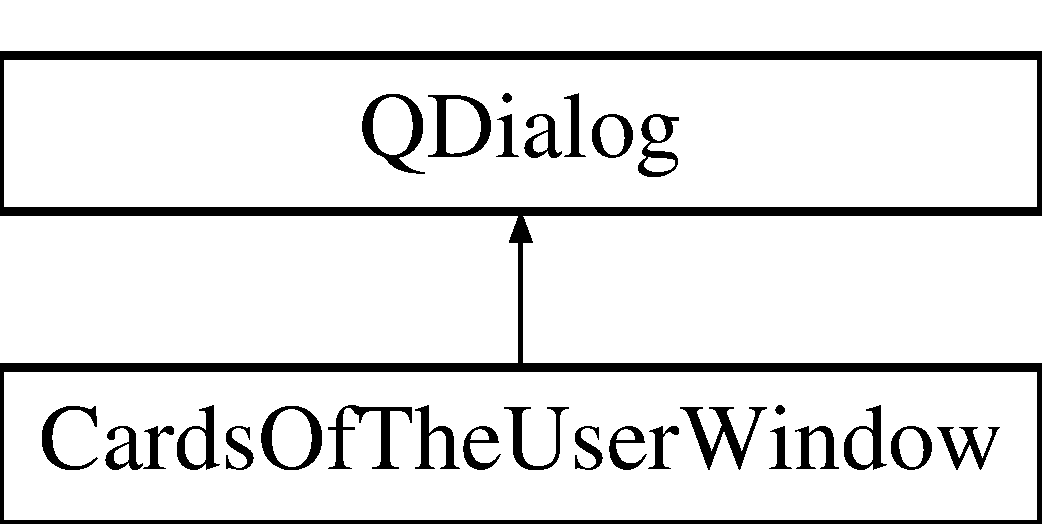
\includegraphics[height=2.000000cm]{classCardsOfTheUserWindow}
\end{center}
\end{figure}
\subsection*{Public Member Functions}
\begin{DoxyCompactItemize}
\item 
\mbox{\Hypertarget{classCardsOfTheUserWindow_a2196040b2451a78b75855244f7ab52e2}\label{classCardsOfTheUserWindow_a2196040b2451a78b75855244f7ab52e2}} 
{\bfseries Cards\+Of\+The\+User\+Window} (\hyperlink{classNewGameCreator}{New\+Game\+Creator} $\ast$new\+Game\+Creator, Q\+Widget $\ast$parent=0)
\end{DoxyCompactItemize}


The documentation for this class was generated from the following files\+:\begin{DoxyCompactItemize}
\item 
gui/Cards\+Of\+The\+User\+Window.\+h\item 
gui/Cards\+Of\+The\+User\+Window.\+cpp\end{DoxyCompactItemize}

\hypertarget{classGame}{}\section{Game Class Reference}
\label{classGame}\index{Game@{Game}}
\subsection*{Public Member Functions}
\begin{DoxyCompactItemize}
\item 
\mbox{\Hypertarget{classGame_af84b325677133cbd7577beb3bfee1425}\label{classGame_af84b325677133cbd7577beb3bfee1425}} 
{\bfseries Game} (\hyperlink{classMainWindow}{Main\+Window} $\ast$main\+Window, int number\+Of\+Players, std\+::vector$<$ Q\+String $>$ player\+Name, std\+::vector$<$ int $>$ player\+Cards\+Number, std\+::vector$<$ Q\+String $>$ user\+Cards)
\item 
\mbox{\Hypertarget{classGame_a95ff1e0758fc07e75ccf98c8f30fb7f0}\label{classGame_a95ff1e0758fc07e75ccf98c8f30fb7f0}} 
void {\bfseries add\+Inquiry} (\hyperlink{classInquiry}{Inquiry} $\ast$q, \hyperlink{classInquiryHistoryWindow}{Inquiry\+History\+Window} $\ast$i)
\item 
\mbox{\Hypertarget{classGame_ac64d371749f3b761b8e73bea994445b8}\label{classGame_ac64d371749f3b761b8e73bea994445b8}} 
std\+::vector$<$ Q\+String $>$ {\bfseries get\+User\+Cards} ()
\item 
\mbox{\Hypertarget{classGame_aa53308fd7e8525ce46834a123fa4da4e}\label{classGame_aa53308fd7e8525ce46834a123fa4da4e}} 
std\+::vector$<$ Q\+String $>$ {\bfseries get\+Room\+Card\+List} ()
\item 
\mbox{\Hypertarget{classGame_a2bb58a8331daae7d32499219fa807dd6}\label{classGame_a2bb58a8331daae7d32499219fa807dd6}} 
std\+::vector$<$ Q\+String $>$ {\bfseries get\+Suspect\+Card\+List} ()
\item 
\mbox{\Hypertarget{classGame_aa419aa078deb35ff55622ab365ac5375}\label{classGame_aa419aa078deb35ff55622ab365ac5375}} 
std\+::vector$<$ Q\+String $>$ {\bfseries get\+Weapon\+Card\+List} ()
\item 
\mbox{\Hypertarget{classGame_abe38ad8f1821220acc48c4568dddbae4}\label{classGame_abe38ad8f1821220acc48c4568dddbae4}} 
std\+::vector$<$ Q\+String $>$ {\bfseries get\+Player\+List} ()
\item 
\mbox{\Hypertarget{classGame_af839571d0f7046e9c92470f12485cf89}\label{classGame_af839571d0f7046e9c92470f12485cf89}} 
int {\bfseries get\+Turn\+Number} ()
\end{DoxyCompactItemize}
\subsection*{Public Attributes}
\begin{DoxyCompactItemize}
\item 
\mbox{\Hypertarget{classGame_a56722c14897977da3ce6f1c943ddf50c}\label{classGame_a56722c14897977da3ce6f1c943ddf50c}} 
std\+::vector$<$ Q\+String $>$ {\bfseries suspect\+Card\+List}
\item 
\mbox{\Hypertarget{classGame_a4a9b27671eb4fb9bfc3009f0d40fb166}\label{classGame_a4a9b27671eb4fb9bfc3009f0d40fb166}} 
std\+::vector$<$ Q\+String $>$ {\bfseries weapon\+Card\+List}
\item 
\mbox{\Hypertarget{classGame_ad5580ea737b17ee1395c4ce1e32fd768}\label{classGame_ad5580ea737b17ee1395c4ce1e32fd768}} 
std\+::vector$<$ Q\+String $>$ {\bfseries room\+Card\+List}
\item 
\mbox{\Hypertarget{classGame_a1ad40bceba6677495abaaff2d93c497e}\label{classGame_a1ad40bceba6677495abaaff2d93c497e}} 
int {\bfseries player\+Number\+Of\+Cards} \mbox{[}$\,$\mbox{]}
\item 
\mbox{\Hypertarget{classGame_a250428392614fc7c7e3f800c5aac9aff}\label{classGame_a250428392614fc7c7e3f800c5aac9aff}} 
int {\bfseries number\+Of\+Players}
\item 
\mbox{\Hypertarget{classGame_a5a6e3c17489efac45233441a0587aff3}\label{classGame_a5a6e3c17489efac45233441a0587aff3}} 
std\+::list$<$ \hyperlink{classInquiry}{Inquiry} $\ast$ $>$ $\ast$ {\bfseries inquiry\+List}
\item 
\mbox{\Hypertarget{classGame_a3adf091eefcc1f00ee02270925b8613e}\label{classGame_a3adf091eefcc1f00ee02270925b8613e}} 
\hyperlink{classPlayer}{Player} {\bfseries player} \mbox{[}6\mbox{]}
\item 
\mbox{\Hypertarget{classGame_a0f4493e06767d8ac4c9b78cfe35b6210}\label{classGame_a0f4493e06767d8ac4c9b78cfe35b6210}} 
std\+::vector$<$ Q\+String $>$ {\bfseries user\+Cards}
\item 
\mbox{\Hypertarget{classGame_a1eea28b69b94947bea0dc07c296f165f}\label{classGame_a1eea28b69b94947bea0dc07c296f165f}} 
std\+::vector$<$ Q\+String $>$ {\bfseries player\+Name}
\item 
\mbox{\Hypertarget{classGame_a8dd6e7ba15211d74ed820475cfc0c1e0}\label{classGame_a8dd6e7ba15211d74ed820475cfc0c1e0}} 
\hyperlink{classMainWindow}{Main\+Window} $\ast$ {\bfseries main\+Window}
\item 
\mbox{\Hypertarget{classGame_a05b65cad55a48f8aa9de08e5ef12da8c}\label{classGame_a05b65cad55a48f8aa9de08e5ef12da8c}} 
int {\bfseries turn\+Number}
\end{DoxyCompactItemize}


The documentation for this class was generated from the following files\+:\begin{DoxyCompactItemize}
\item 
game/Game.\+h\item 
game/Game.\+cpp\end{DoxyCompactItemize}

\hypertarget{classGameWindow}{}\section{Game\+Window Class Reference}
\label{classGameWindow}\index{Game\+Window@{Game\+Window}}
Inheritance diagram for Game\+Window\+:\begin{figure}[H]
\begin{center}
\leavevmode
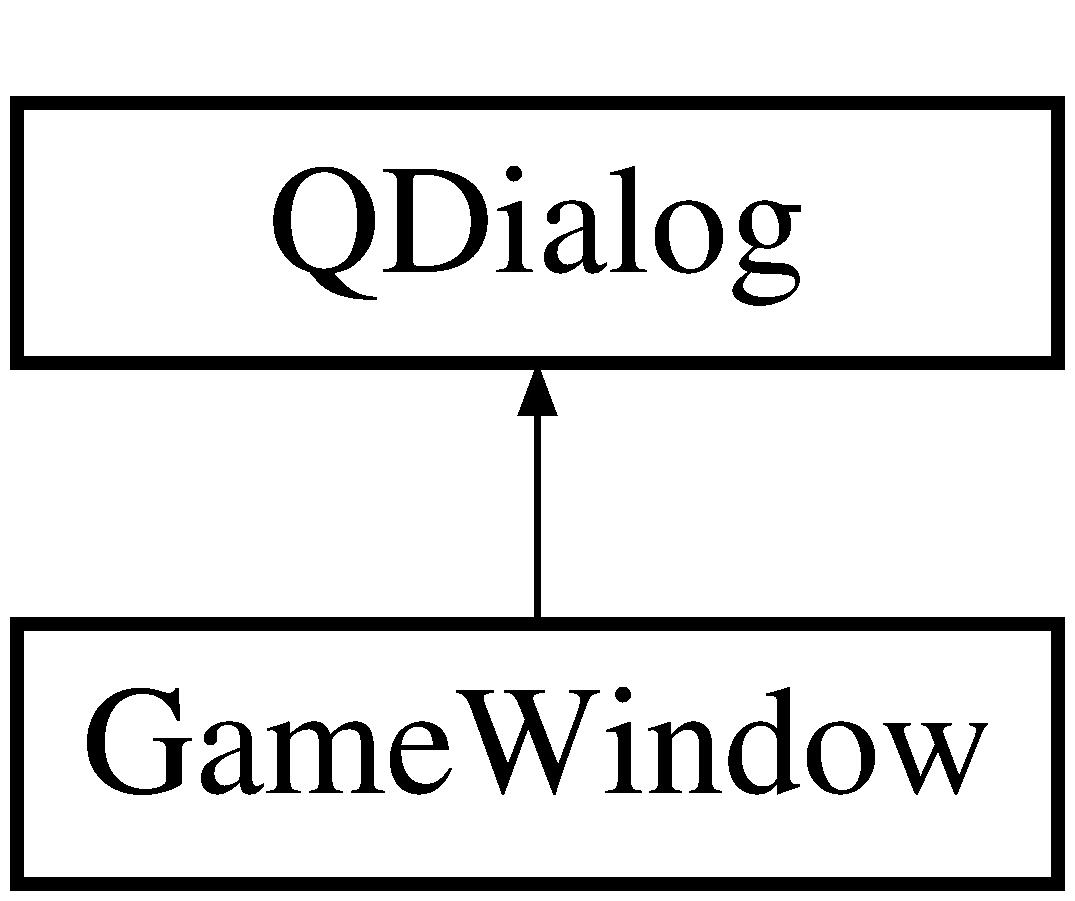
\includegraphics[height=2.000000cm]{classGameWindow}
\end{center}
\end{figure}
\subsection*{Public Member Functions}
\begin{DoxyCompactItemize}
\item 
\mbox{\Hypertarget{classGameWindow_af2794433e83e7821746b6c8821772ebc}\label{classGameWindow_af2794433e83e7821746b6c8821772ebc}} 
{\bfseries Game\+Window} (\hyperlink{classGame}{Game} $\ast$game, Q\+Widget $\ast$parent=0)
\item 
\mbox{\Hypertarget{classGameWindow_a4cb00162e90812c2331d1a28ba0b0ebc}\label{classGameWindow_a4cb00162e90812c2331d1a28ba0b0ebc}} 
void {\bfseries myupdate} ()
\item 
\mbox{\Hypertarget{classGameWindow_a3506333aeaf3d6e79ec07e3cc20ff21a}\label{classGameWindow_a3506333aeaf3d6e79ec07e3cc20ff21a}} 
void {\bfseries update\+Card\+Table} (Q\+String card, Q\+String player, Q\+String value)
\item 
\mbox{\Hypertarget{classGameWindow_ac978d7204e47e584a385a3c60d83dd8a}\label{classGameWindow_ac978d7204e47e584a385a3c60d83dd8a}} 
void {\bfseries close\+Event} (Q\+Close\+Event $\ast$e)
\item 
\mbox{\Hypertarget{classGameWindow_a8dc0b395836425a0f20bde22293b4075}\label{classGameWindow_a8dc0b395836425a0f20bde22293b4075}} 
void {\bfseries myupdate2} ()
\end{DoxyCompactItemize}
\subsection*{Public Attributes}
\begin{DoxyCompactItemize}
\item 
\mbox{\Hypertarget{classGameWindow_a83490ef95c69897b92002b3016de98c9}\label{classGameWindow_a83490ef95c69897b92002b3016de98c9}} 
\hyperlink{classGame}{Game} $\ast$ {\bfseries game}
\item 
\mbox{\Hypertarget{classGameWindow_a4e7d69a2995175c4a7ebaa2cf082ad1b}\label{classGameWindow_a4e7d69a2995175c4a7ebaa2cf082ad1b}} 
Q\+Table\+Widget $\ast$ {\bfseries room\+Card\+Table}
\end{DoxyCompactItemize}


The documentation for this class was generated from the following files\+:\begin{DoxyCompactItemize}
\item 
gui/Game\+Window.\+h\item 
gui/Game\+Window.\+cpp\end{DoxyCompactItemize}

\hypertarget{classInquiry}{}\section{Inquiry Class Reference}
\label{classInquiry}\index{Inquiry@{Inquiry}}
\subsection*{Public Member Functions}
\begin{DoxyCompactItemize}
\item 
\mbox{\Hypertarget{classInquiry_ae4001d759383bd9c5220ee8ea4e3f5d1}\label{classInquiry_ae4001d759383bd9c5220ee8ea4e3f5d1}} 
{\bfseries Inquiry} (int turn, std\+::string inquirer, std\+::string room, std\+::string suspect, std\+::string weapon, std\+::string giver)
\end{DoxyCompactItemize}
\subsection*{Public Attributes}
\begin{DoxyCompactItemize}
\item 
\mbox{\Hypertarget{classInquiry_ad8cd9223fe302565184aa7737bda9472}\label{classInquiry_ad8cd9223fe302565184aa7737bda9472}} 
int {\bfseries turn}
\item 
\mbox{\Hypertarget{classInquiry_a8eb1063b395f7cab0979e146093cb650}\label{classInquiry_a8eb1063b395f7cab0979e146093cb650}} 
std\+::string {\bfseries inquirer}
\item 
\mbox{\Hypertarget{classInquiry_ace3d8a33144bf20b9b7c07921868af38}\label{classInquiry_ace3d8a33144bf20b9b7c07921868af38}} 
std\+::string {\bfseries giver}
\item 
\mbox{\Hypertarget{classInquiry_a8ed4b7a6b7c7a030eb137e1eea8c5697}\label{classInquiry_a8ed4b7a6b7c7a030eb137e1eea8c5697}} 
std\+::string {\bfseries room}
\item 
\mbox{\Hypertarget{classInquiry_ad6d0ea284f6b62e5a4119e93cd77749b}\label{classInquiry_ad6d0ea284f6b62e5a4119e93cd77749b}} 
std\+::string {\bfseries suspect}
\item 
\mbox{\Hypertarget{classInquiry_ac34775cd7cc0f05f210158d2ce33fa98}\label{classInquiry_ac34775cd7cc0f05f210158d2ce33fa98}} 
std\+::string {\bfseries weapon}
\end{DoxyCompactItemize}


The documentation for this class was generated from the following files\+:\begin{DoxyCompactItemize}
\item 
game/Inquiry.\+h\item 
game/Inquiry.\+cpp\end{DoxyCompactItemize}

\hypertarget{classInquiryHistoryWindow}{}\section{Inquiry\+History\+Window Class Reference}
\label{classInquiryHistoryWindow}\index{Inquiry\+History\+Window@{Inquiry\+History\+Window}}
Inheritance diagram for Inquiry\+History\+Window\+:\begin{figure}[H]
\begin{center}
\leavevmode
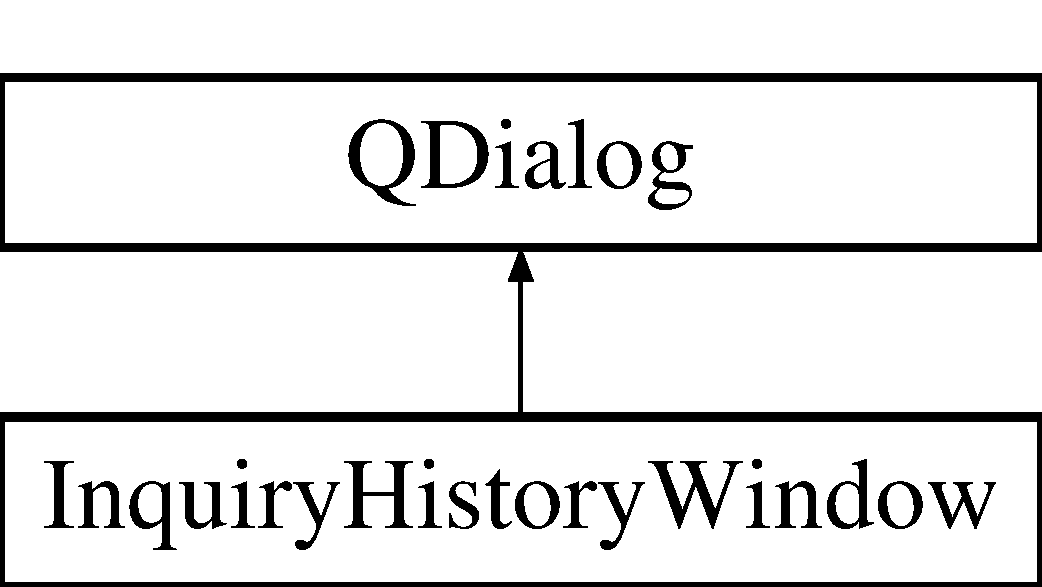
\includegraphics[height=2.000000cm]{classInquiryHistoryWindow}
\end{center}
\end{figure}
\subsection*{Public Member Functions}
\begin{DoxyCompactItemize}
\item 
\mbox{\Hypertarget{classInquiryHistoryWindow_a9a590b61cb46dfbaf2062defd4ecc1a3}\label{classInquiryHistoryWindow_a9a590b61cb46dfbaf2062defd4ecc1a3}} 
{\bfseries Inquiry\+History\+Window} (\hyperlink{classGame}{Game} $\ast$g, Q\+Widget $\ast$parent=0)
\item 
\mbox{\Hypertarget{classInquiryHistoryWindow_a38d5323261a7ba223517235f608fcae6}\label{classInquiryHistoryWindow_a38d5323261a7ba223517235f608fcae6}} 
void {\bfseries close\+Event} (Q\+Close\+Event $\ast$e)
\item 
\mbox{\Hypertarget{classInquiryHistoryWindow_ac57591d79ca9911cd085d80411a7d440}\label{classInquiryHistoryWindow_ac57591d79ca9911cd085d80411a7d440}} 
void {\bfseries myupdate} ()
\end{DoxyCompactItemize}
\subsection*{Public Attributes}
\begin{DoxyCompactItemize}
\item 
\mbox{\Hypertarget{classInquiryHistoryWindow_ad3c99570687772e595bffd9160678471}\label{classInquiryHistoryWindow_ad3c99570687772e595bffd9160678471}} 
\hyperlink{classGame}{Game} $\ast$ {\bfseries g}
\item 
\mbox{\Hypertarget{classInquiryHistoryWindow_a21f2011f43eadd1c236ba1ffc6a035ae}\label{classInquiryHistoryWindow_a21f2011f43eadd1c236ba1ffc6a035ae}} 
Q\+Table\+Widget $\ast$ {\bfseries inquiry\+History\+Table}
\end{DoxyCompactItemize}


The documentation for this class was generated from the following files\+:\begin{DoxyCompactItemize}
\item 
gui/Inquiry\+History\+Window.\+h\item 
gui/Inquiry\+History\+Window.\+cpp\end{DoxyCompactItemize}

\hypertarget{classMainWindow}{}\section{Main\+Window Class Reference}
\label{classMainWindow}\index{Main\+Window@{Main\+Window}}
Inheritance diagram for Main\+Window\+:\begin{figure}[H]
\begin{center}
\leavevmode
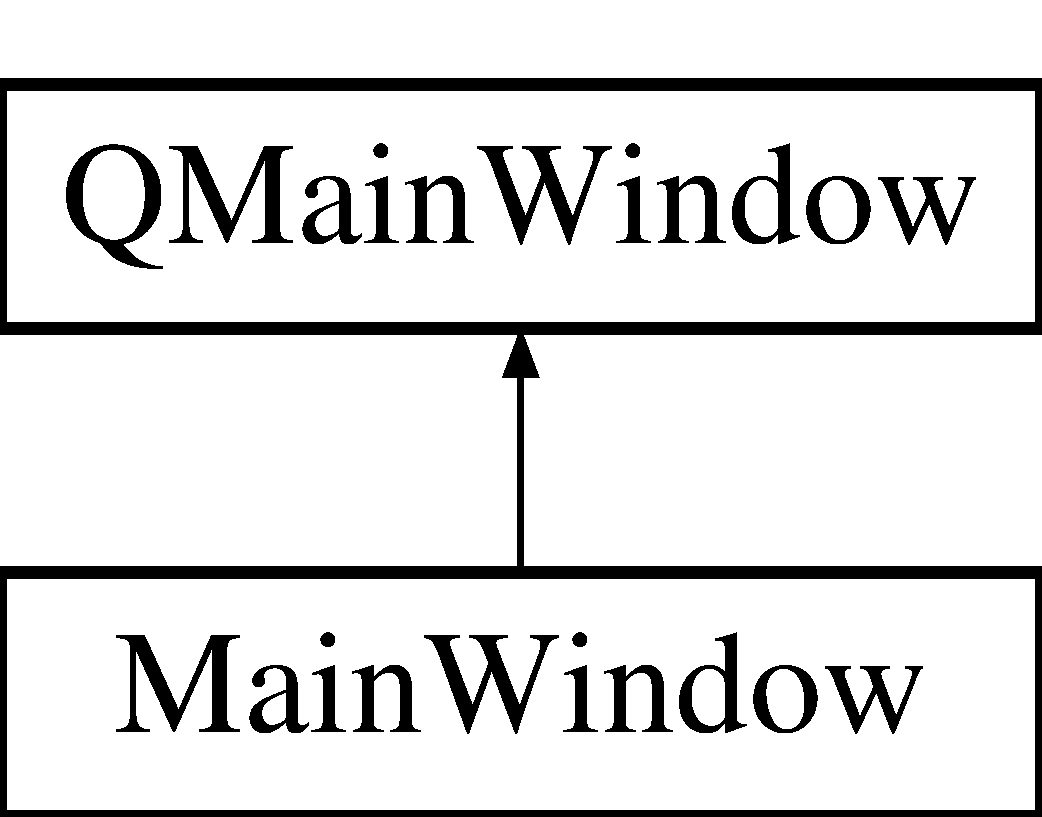
\includegraphics[height=2.000000cm]{classMainWindow}
\end{center}
\end{figure}
\subsection*{Public Member Functions}
\begin{DoxyCompactItemize}
\item 
\mbox{\Hypertarget{classMainWindow_a6d00d0c625db7096f416034d07ba1acd}\label{classMainWindow_a6d00d0c625db7096f416034d07ba1acd}} 
{\bfseries Main\+Window} (\hyperlink{classMain}{Main} $\ast$main, Q\+Widget $\ast$parent=0)
\item 
\mbox{\Hypertarget{classMainWindow_ae12f8f63791595567b6250f8bb002bda}\label{classMainWindow_ae12f8f63791595567b6250f8bb002bda}} 
void {\bfseries resize\+Event} (Q\+Resize\+Event $\ast$event)
\item 
\mbox{\Hypertarget{classMainWindow_a889d39caf6b396921d972800e2fba819}\label{classMainWindow_a889d39caf6b396921d972800e2fba819}} 
void {\bfseries set\+Subwindow} (Q\+Widget $\ast$q)
\item 
\mbox{\Hypertarget{classMainWindow_aa8bd15bfe653d4a823453aa2de06b807}\label{classMainWindow_aa8bd15bfe653d4a823453aa2de06b807}} 
void {\bfseries create\+New\+Game} ()
\item 
\mbox{\Hypertarget{classMainWindow_a33c0c4b08a759f5c32446d284a811947}\label{classMainWindow_a33c0c4b08a759f5c32446d284a811947}} 
void {\bfseries set\+Game} (\hyperlink{classGame}{Game} $\ast$game)
\item 
\mbox{\Hypertarget{classMainWindow_aa78b3f5e5a1226396581fde03f7f1172}\label{classMainWindow_aa78b3f5e5a1226396581fde03f7f1172}} 
void {\bfseries myupdate} ()
\end{DoxyCompactItemize}
\subsection*{Public Attributes}
\begin{DoxyCompactItemize}
\item 
\mbox{\Hypertarget{classMainWindow_a0df1000428a75f4b5ca749b84f1f4a28}\label{classMainWindow_a0df1000428a75f4b5ca749b84f1f4a28}} 
Q\+Pixmap $\ast$ {\bfseries m\+\_\+p\+Pixmap}
\item 
\mbox{\Hypertarget{classMainWindow_a4687ca985e01079dd109899fa997b5ef}\label{classMainWindow_a4687ca985e01079dd109899fa997b5ef}} 
Q\+Palette $\ast$ {\bfseries m\+\_\+p\+Palette}
\end{DoxyCompactItemize}


The documentation for this class was generated from the following files\+:\begin{DoxyCompactItemize}
\item 
gui/Main\+Window.\+h\item 
gui/Main\+Window.\+cpp\end{DoxyCompactItemize}

\hypertarget{classNamesOfThePlayersWindow}{}\section{Names\+Of\+The\+Players\+Window Class Reference}
\label{classNamesOfThePlayersWindow}\index{Names\+Of\+The\+Players\+Window@{Names\+Of\+The\+Players\+Window}}
Inheritance diagram for Names\+Of\+The\+Players\+Window\+:\begin{figure}[H]
\begin{center}
\leavevmode
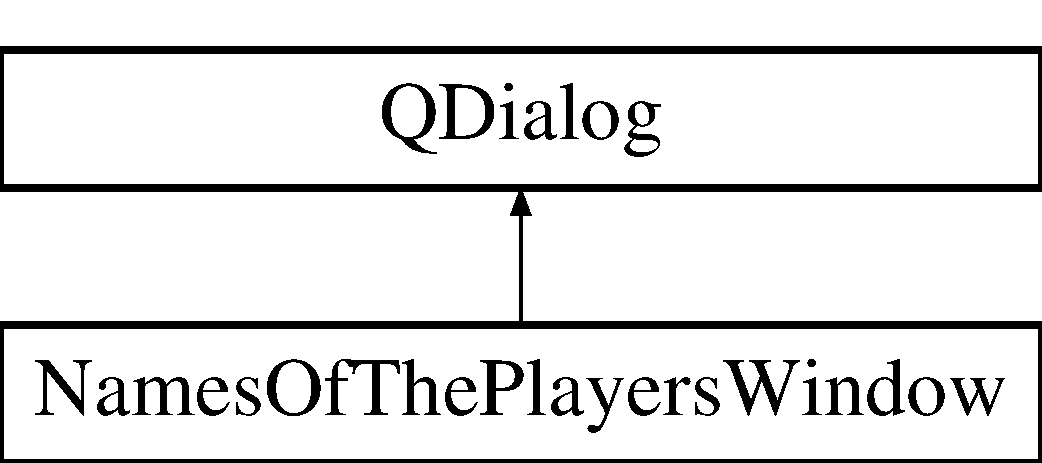
\includegraphics[height=3.000000cm]{classNamesOfThePlayersWindow}
\end{center}
\end{figure}
\subsection*{Public Slots}
\begin{DoxyCompactItemize}
\item 
\mbox{\Hypertarget{classNamesOfThePlayersWindow_ac52d684884838cb8f99a495b3c0f89d9}\label{classNamesOfThePlayersWindow_ac52d684884838cb8f99a495b3c0f89d9}} 
void {\bfseries enable\+Or\+Disable\+Confirm\+Button} (const Q\+String \&text)
\end{DoxyCompactItemize}
\subsection*{Public Member Functions}
\begin{DoxyCompactItemize}
\item 
\mbox{\Hypertarget{classNamesOfThePlayersWindow_a199b485baab3f42c072a33e845cd35cf}\label{classNamesOfThePlayersWindow_a199b485baab3f42c072a33e845cd35cf}} 
{\bfseries Names\+Of\+The\+Players\+Window} (\hyperlink{classNewGameCreator}{New\+Game\+Creator} $\ast$new\+Game\+Creator, Q\+Widget $\ast$parent=0)
\end{DoxyCompactItemize}
\subsection*{Additional Inherited Members}


The documentation for this class was generated from the following files\+:\begin{DoxyCompactItemize}
\item 
gui/Names\+Of\+The\+Players\+Window.\+h\item 
gui/Names\+Of\+The\+Players\+Window.\+cpp\end{DoxyCompactItemize}

\hypertarget{classNewGameCreationWindow}{}\section{New\+Game\+Creation\+Window Class Reference}
\label{classNewGameCreationWindow}\index{New\+Game\+Creation\+Window@{New\+Game\+Creation\+Window}}


Parent class of windows used to create a new game.  




{\ttfamily \#include $<$New\+Game\+Creation\+Window.\+h$>$}

Inheritance diagram for New\+Game\+Creation\+Window\+:\begin{figure}[H]
\begin{center}
\leavevmode
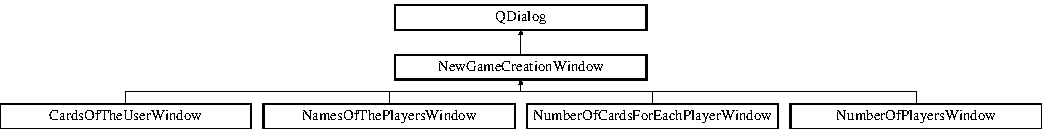
\includegraphics[height=3.000000cm]{classNewGameCreationWindow}
\end{center}
\end{figure}
\subsection*{Public Member Functions}
\begin{DoxyCompactItemize}
\item 
\hyperlink{classNewGameCreationWindow_a1b8cd9166289a086a951c2ee9d6bfebe}{New\+Game\+Creation\+Window} (Q\+Widget $\ast$parent=0)
\begin{DoxyCompactList}\small\item\em Create the window. \end{DoxyCompactList}\end{DoxyCompactItemize}


\subsection{Detailed Description}
Parent class of windows used to create a new game. 

This class is the parent of all the windows that are used to create a new game. It is a Q\+Dialog to center it and it is modal to avoid that the user, when one of the children windows of this class is opened, does something else than inserting the data required by the children window. 

\subsection{Constructor \& Destructor Documentation}
\mbox{\Hypertarget{classNewGameCreationWindow_a1b8cd9166289a086a951c2ee9d6bfebe}\label{classNewGameCreationWindow_a1b8cd9166289a086a951c2ee9d6bfebe}} 
\index{New\+Game\+Creation\+Window@{New\+Game\+Creation\+Window}!New\+Game\+Creation\+Window@{New\+Game\+Creation\+Window}}
\index{New\+Game\+Creation\+Window@{New\+Game\+Creation\+Window}!New\+Game\+Creation\+Window@{New\+Game\+Creation\+Window}}
\subsubsection{\texorpdfstring{New\+Game\+Creation\+Window()}{NewGameCreationWindow()}}
{\footnotesize\ttfamily New\+Game\+Creation\+Window\+::\+New\+Game\+Creation\+Window (\begin{DoxyParamCaption}\item[{Q\+Widget $\ast$}]{parent = {\ttfamily 0} }\end{DoxyParamCaption})}



Create the window. 


\begin{DoxyParams}{Parameters}
{\em parent} & the parent of the window\\
\hline
\end{DoxyParams}
Create the window and set it to be modal. 

The documentation for this class was generated from the following files\+:\begin{DoxyCompactItemize}
\item 
gui/New\+Game\+Creation\+Window.\+h\item 
gui/New\+Game\+Creation\+Window.\+cpp\end{DoxyCompactItemize}

\hypertarget{classNewGameCreator}{}\section{New\+Game\+Creator Class Reference}
\label{classNewGameCreator}\index{New\+Game\+Creator@{New\+Game\+Creator}}
\subsection*{Public Member Functions}
\begin{DoxyCompactItemize}
\item 
\mbox{\Hypertarget{classNewGameCreator_a30b53bdda90bbf9f9ce8183e6e475274}\label{classNewGameCreator_a30b53bdda90bbf9f9ce8183e6e475274}} 
{\bfseries New\+Game\+Creator} (\hyperlink{classMainWindow}{Main\+Window} $\ast$main\+Window)
\item 
\mbox{\Hypertarget{classNewGameCreator_aa3cc740c81a3264a352a9cac2a2c60eb}\label{classNewGameCreator_aa3cc740c81a3264a352a9cac2a2c60eb}} 
void {\bfseries open\+Next\+Window} ()
\item 
\mbox{\Hypertarget{classNewGameCreator_a6118892cee025ca10e05741387ce999c}\label{classNewGameCreator_a6118892cee025ca10e05741387ce999c}} 
void {\bfseries set\+Number\+Of\+Players} (int number\+Of\+Players)
\item 
\mbox{\Hypertarget{classNewGameCreator_acc48dac51f9b7cf2b2b6793f321ce144}\label{classNewGameCreator_acc48dac51f9b7cf2b2b6793f321ce144}} 
int {\bfseries get\+Number\+Of\+Players} ()
\item 
\mbox{\Hypertarget{classNewGameCreator_a753d5ed531a6d57ed1418a696c66ddb2}\label{classNewGameCreator_a753d5ed531a6d57ed1418a696c66ddb2}} 
void {\bfseries set\+Names\+Of\+The\+Players} (std\+::vector$<$ Q\+String $>$ player\+Name)
\item 
\mbox{\Hypertarget{classNewGameCreator_a1aac05c21a10a7e4709c831ac6e56b91}\label{classNewGameCreator_a1aac05c21a10a7e4709c831ac6e56b91}} 
std\+::vector$<$ Q\+String $>$ {\bfseries get\+Names\+Of\+The\+Players} ()
\item 
\mbox{\Hypertarget{classNewGameCreator_abff5d40e11ad39ab4356af6717d88e83}\label{classNewGameCreator_abff5d40e11ad39ab4356af6717d88e83}} 
void {\bfseries set\+Number\+Of\+Cards\+For\+Each\+Player} (std\+::vector$<$ int $>$ player\+Cards\+Number)
\item 
\mbox{\Hypertarget{classNewGameCreator_a14244649f919d6946d33c518932105f3}\label{classNewGameCreator_a14244649f919d6946d33c518932105f3}} 
void {\bfseries set\+Cards\+Of\+The\+User} (std\+::vector$<$ Q\+String $>$ user\+Cards)
\item 
\mbox{\Hypertarget{classNewGameCreator_ac2905e16676010c2989674a8e18e2d9b}\label{classNewGameCreator_ac2905e16676010c2989674a8e18e2d9b}} 
std\+::vector$<$ Q\+String $>$ {\bfseries get\+Cards\+Of\+The\+User} ()
\item 
\mbox{\Hypertarget{classNewGameCreator_a6bdc7ce36cc5c1bf2952ddd0167e6681}\label{classNewGameCreator_a6bdc7ce36cc5c1bf2952ddd0167e6681}} 
std\+::vector$<$ int $>$ {\bfseries get\+Number\+Of\+Cards\+For\+Each\+Player} ()
\end{DoxyCompactItemize}
\subsection*{Private Attributes}
\begin{DoxyCompactItemize}
\item 
\mbox{\Hypertarget{classNewGameCreator_ad6c9525b56ae5262e001234963134eed}\label{classNewGameCreator_ad6c9525b56ae5262e001234963134eed}} 
int {\bfseries number\+Of\+Opened\+Windows}
\item 
\mbox{\Hypertarget{classNewGameCreator_a04cf8166bfa23a8b42af83fdf7aba40b}\label{classNewGameCreator_a04cf8166bfa23a8b42af83fdf7aba40b}} 
\hyperlink{classGame}{Game} $\ast$ {\bfseries game}
\item 
\mbox{\Hypertarget{classNewGameCreator_aefa06e71c9f9fb3112daba05eeba7766}\label{classNewGameCreator_aefa06e71c9f9fb3112daba05eeba7766}} 
\hyperlink{classMainWindow}{Main\+Window} $\ast$ {\bfseries main\+Window}
\item 
\mbox{\Hypertarget{classNewGameCreator_ac915dc1d2da341179a23ec805f94de9f}\label{classNewGameCreator_ac915dc1d2da341179a23ec805f94de9f}} 
int {\bfseries number\+Of\+Players}
\item 
\mbox{\Hypertarget{classNewGameCreator_ae916a350032c1a8ad794e92082fb3b3c}\label{classNewGameCreator_ae916a350032c1a8ad794e92082fb3b3c}} 
std\+::vector$<$ Q\+String $>$ {\bfseries player\+Name}
\item 
\mbox{\Hypertarget{classNewGameCreator_a4d126ba7155fc11d1f801be52fe6152d}\label{classNewGameCreator_a4d126ba7155fc11d1f801be52fe6152d}} 
std\+::vector$<$ int $>$ {\bfseries player\+Cards\+Number}
\item 
\mbox{\Hypertarget{classNewGameCreator_afe39c8c4ae8bff26abff92bbf692265c}\label{classNewGameCreator_afe39c8c4ae8bff26abff92bbf692265c}} 
std\+::vector$<$ Q\+String $>$ {\bfseries user\+Cards}
\end{DoxyCompactItemize}


The documentation for this class was generated from the following files\+:\begin{DoxyCompactItemize}
\item 
game/New\+Game\+Creator.\+h\item 
game/New\+Game\+Creator.\+cpp\end{DoxyCompactItemize}

\hypertarget{classNewInquiryWindow}{}\section{New\+Inquiry\+Window Class Reference}
\label{classNewInquiryWindow}\index{New\+Inquiry\+Window@{New\+Inquiry\+Window}}
Inheritance diagram for New\+Inquiry\+Window\+:\begin{figure}[H]
\begin{center}
\leavevmode
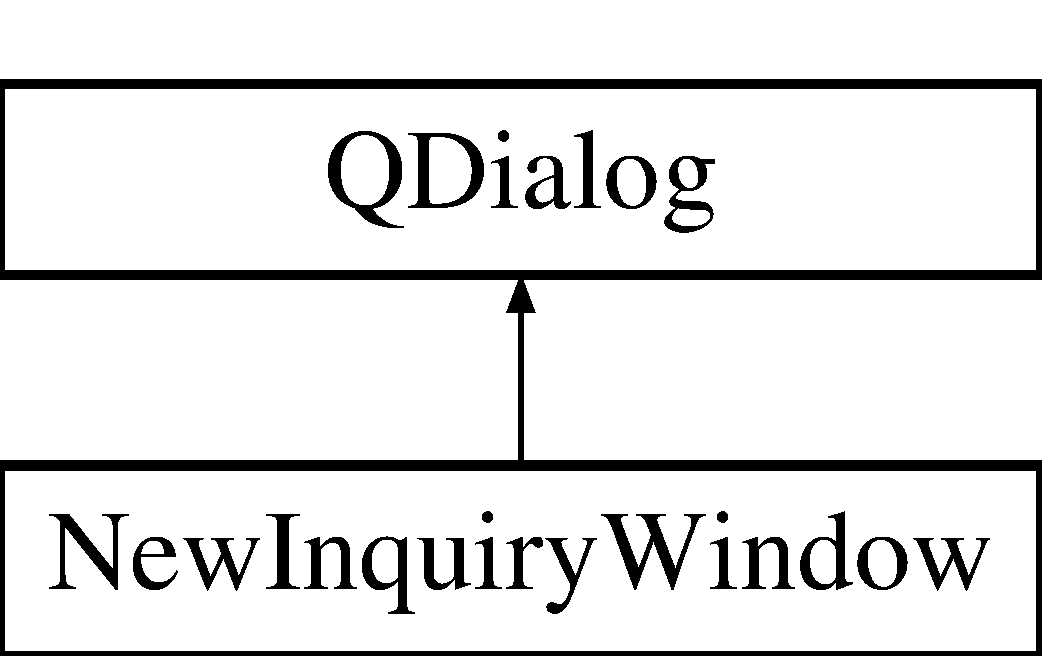
\includegraphics[height=2.000000cm]{classNewInquiryWindow}
\end{center}
\end{figure}
\subsection*{Public Slots}
\begin{DoxyCompactItemize}
\item 
\mbox{\Hypertarget{classNewInquiryWindow_aa8d01ffe4f4dc704505785f507652bd2}\label{classNewInquiryWindow_aa8d01ffe4f4dc704505785f507652bd2}} 
void {\bfseries open\+New\+Window} ()
\end{DoxyCompactItemize}
\subsection*{Public Member Functions}
\begin{DoxyCompactItemize}
\item 
\mbox{\Hypertarget{classNewInquiryWindow_a1fb15d4ea79c5b3c8c81b2e523eeffa8}\label{classNewInquiryWindow_a1fb15d4ea79c5b3c8c81b2e523eeffa8}} 
{\bfseries New\+Inquiry\+Window} (\hyperlink{classGame}{Game} $\ast$g, \hyperlink{classInquiryHistoryWindow}{Inquiry\+History\+Window} $\ast$i, Q\+Widget $\ast$parent=0)
\end{DoxyCompactItemize}
\subsection*{Public Attributes}
\begin{DoxyCompactItemize}
\item 
\mbox{\Hypertarget{classNewInquiryWindow_a76c564bfdd2a2950d4190e0d7b55091e}\label{classNewInquiryWindow_a76c564bfdd2a2950d4190e0d7b55091e}} 
\hyperlink{classGame}{Game} $\ast$ {\bfseries game}
\item 
\mbox{\Hypertarget{classNewInquiryWindow_a78a6436a76286c46819f4c3c4b42b2be}\label{classNewInquiryWindow_a78a6436a76286c46819f4c3c4b42b2be}} 
\hyperlink{classGameWindow}{Game\+Window} $\ast$ {\bfseries gw}
\end{DoxyCompactItemize}
\subsection*{Private Slots}
\begin{DoxyCompactItemize}
\item 
\mbox{\Hypertarget{classNewInquiryWindow_ab4988cfb69c9f9a851359fc3490cd790}\label{classNewInquiryWindow_ab4988cfb69c9f9a851359fc3490cd790}} 
void {\bfseries mydo} ()
\end{DoxyCompactItemize}
\subsection*{Private Member Functions}
\begin{DoxyCompactItemize}
\item 
\mbox{\Hypertarget{classNewInquiryWindow_a9acb35a5231d8a493989c456c83c7640}\label{classNewInquiryWindow_a9acb35a5231d8a493989c456c83c7640}} 
void {\bfseries close\+Event} (Q\+Close\+Event $\ast$e)
\end{DoxyCompactItemize}
\subsection*{Private Attributes}
\begin{DoxyCompactItemize}
\item 
\mbox{\Hypertarget{classNewInquiryWindow_a319dfc303bf61850e2cddf3a3b81a25d}\label{classNewInquiryWindow_a319dfc303bf61850e2cddf3a3b81a25d}} 
Q\+Radio\+Button $\ast$ {\bfseries caller\+Radio\+Button} \mbox{[}6\mbox{]}
\item 
\mbox{\Hypertarget{classNewInquiryWindow_a8232406fc1ba3183c0b4408aac004b50}\label{classNewInquiryWindow_a8232406fc1ba3183c0b4408aac004b50}} 
Q\+Radio\+Button $\ast$ {\bfseries room\+Card\+Check\+Box} \mbox{[}10\mbox{]}
\item 
\mbox{\Hypertarget{classNewInquiryWindow_a3a7ea514cbe1d9bdf0bf53495cfdbf96}\label{classNewInquiryWindow_a3a7ea514cbe1d9bdf0bf53495cfdbf96}} 
Q\+Radio\+Button $\ast$ {\bfseries suspect\+Card\+Check\+Box} \mbox{[}6\mbox{]}
\item 
\mbox{\Hypertarget{classNewInquiryWindow_acb6f1af5af3b523574bb8f1f055ad6ec}\label{classNewInquiryWindow_acb6f1af5af3b523574bb8f1f055ad6ec}} 
Q\+Radio\+Button $\ast$ {\bfseries weapon\+Card\+Check\+Box} \mbox{[}6\mbox{]}
\item 
\mbox{\Hypertarget{classNewInquiryWindow_a1aff2e998cbd0b11dde2f65c601e6e4d}\label{classNewInquiryWindow_a1aff2e998cbd0b11dde2f65c601e6e4d}} 
Q\+Radio\+Button $\ast$ {\bfseries giver\+Radio\+Button} \mbox{[}7\mbox{]}
\item 
\mbox{\Hypertarget{classNewInquiryWindow_ac87190201e47b7c553007580e864b5cd}\label{classNewInquiryWindow_ac87190201e47b7c553007580e864b5cd}} 
\hyperlink{classInquiryHistoryWindow}{Inquiry\+History\+Window} $\ast$ {\bfseries i}
\end{DoxyCompactItemize}


The documentation for this class was generated from the following files\+:\begin{DoxyCompactItemize}
\item 
gui/New\+Inquiry\+Window.\+h\item 
gui/New\+Inquiry\+Window.\+cpp\end{DoxyCompactItemize}

\hypertarget{classNumberOfCardsForEachPlayerWindow}{}\section{Number\+Of\+Cards\+For\+Each\+Player\+Window Class Reference}
\label{classNumberOfCardsForEachPlayerWindow}\index{Number\+Of\+Cards\+For\+Each\+Player\+Window@{Number\+Of\+Cards\+For\+Each\+Player\+Window}}
Inheritance diagram for Number\+Of\+Cards\+For\+Each\+Player\+Window\+:\begin{figure}[H]
\begin{center}
\leavevmode
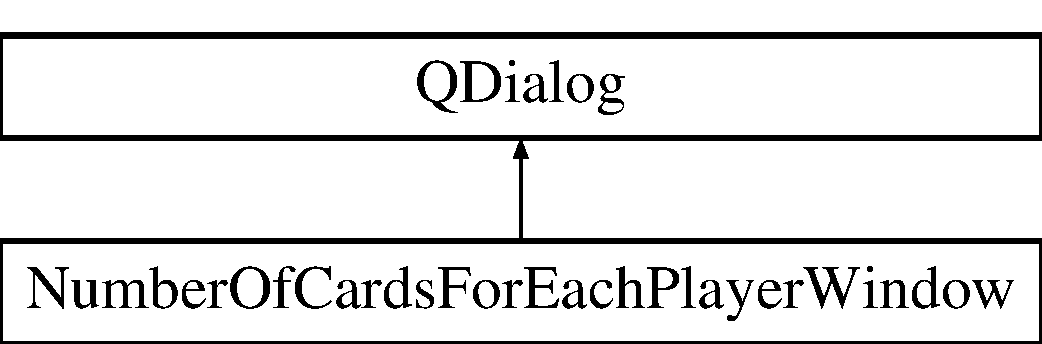
\includegraphics[height=2.000000cm]{classNumberOfCardsForEachPlayerWindow}
\end{center}
\end{figure}
\subsection*{Public Member Functions}
\begin{DoxyCompactItemize}
\item 
\mbox{\Hypertarget{classNumberOfCardsForEachPlayerWindow_aadd6710e807d6ac5a401c1ecbe51792b}\label{classNumberOfCardsForEachPlayerWindow_aadd6710e807d6ac5a401c1ecbe51792b}} 
{\bfseries Number\+Of\+Cards\+For\+Each\+Player\+Window} (\hyperlink{classNewGameCreator}{New\+Game\+Creator} $\ast$new\+Game\+Creator, Q\+Widget $\ast$parent=0)
\end{DoxyCompactItemize}
\subsection*{Private Slots}
\begin{DoxyCompactItemize}
\item 
\mbox{\Hypertarget{classNumberOfCardsForEachPlayerWindow_a0f9c2e3e60b2833382ebed28944666ee}\label{classNumberOfCardsForEachPlayerWindow_a0f9c2e3e60b2833382ebed28944666ee}} 
void {\bfseries open\+Next\+Window} ()
\end{DoxyCompactItemize}
\subsection*{Private Member Functions}
\begin{DoxyCompactItemize}
\item 
\mbox{\Hypertarget{classNumberOfCardsForEachPlayerWindow_ac88a653ee30726209ba3b7e97095f091}\label{classNumberOfCardsForEachPlayerWindow_ac88a653ee30726209ba3b7e97095f091}} 
Q\+Group\+Box $\ast$ {\bfseries create\+Number\+Of\+Players\+Group} ()
\end{DoxyCompactItemize}
\subsection*{Private Attributes}
\begin{DoxyCompactItemize}
\item 
\mbox{\Hypertarget{classNumberOfCardsForEachPlayerWindow_af3017a12939983c5af2a5f1f93e692bd}\label{classNumberOfCardsForEachPlayerWindow_af3017a12939983c5af2a5f1f93e692bd}} 
\hyperlink{classNewGameCreator}{New\+Game\+Creator} $\ast$ {\bfseries new\+Game\+Creator}
\item 
\mbox{\Hypertarget{classNumberOfCardsForEachPlayerWindow_afe54ffe51625a918a333b128970d8551}\label{classNumberOfCardsForEachPlayerWindow_afe54ffe51625a918a333b128970d8551}} 
Q\+Push\+Button $\ast$ {\bfseries m\+\_\+button}
\item 
\mbox{\Hypertarget{classNumberOfCardsForEachPlayerWindow_a2b91b133fa4890d55226786b17a187d2}\label{classNumberOfCardsForEachPlayerWindow_a2b91b133fa4890d55226786b17a187d2}} 
int {\bfseries non\+Empty\+Name} \mbox{[}6\mbox{]}
\item 
\mbox{\Hypertarget{classNumberOfCardsForEachPlayerWindow_a1a0ac0b68c880c24feaf78dd49f6fa4b}\label{classNumberOfCardsForEachPlayerWindow_a1a0ac0b68c880c24feaf78dd49f6fa4b}} 
int {\bfseries non\+Empty\+Names} = 0
\item 
\mbox{\Hypertarget{classNumberOfCardsForEachPlayerWindow_a3cb54ea3de541699a4e56c5efe57a817}\label{classNumberOfCardsForEachPlayerWindow_a3cb54ea3de541699a4e56c5efe57a817}} 
Q\+Hash$<$ Q\+Line\+Edit $\ast$$\ast$, int $>$ {\bfseries hash}
\item 
\mbox{\Hypertarget{classNumberOfCardsForEachPlayerWindow_a7fa0fd165d852722cc48c61cee4afc14}\label{classNumberOfCardsForEachPlayerWindow_a7fa0fd165d852722cc48c61cee4afc14}} 
Q\+Line\+Edit $\ast$ {\bfseries player\+Name\+Line\+Edit} \mbox{[}6\mbox{]}
\item 
\mbox{\Hypertarget{classNumberOfCardsForEachPlayerWindow_a57fa2226d488288ed87844a700b6b86e}\label{classNumberOfCardsForEachPlayerWindow_a57fa2226d488288ed87844a700b6b86e}} 
Q\+Label $\ast$ {\bfseries player\+Name\+Label} \mbox{[}6\mbox{]}
\item 
\mbox{\Hypertarget{classNumberOfCardsForEachPlayerWindow_adfc43631d8f3c202b5d3209438c3efba}\label{classNumberOfCardsForEachPlayerWindow_adfc43631d8f3c202b5d3209438c3efba}} 
\hyperlink{classMainWindow}{Main\+Window} $\ast$ {\bfseries main\+Window}
\item 
\mbox{\Hypertarget{classNumberOfCardsForEachPlayerWindow_abda07ceae6819be7b8f648acc1b503ad}\label{classNumberOfCardsForEachPlayerWindow_abda07ceae6819be7b8f648acc1b503ad}} 
std\+::vector$<$ Q\+String $>$ {\bfseries player\+Name}
\item 
\mbox{\Hypertarget{classNumberOfCardsForEachPlayerWindow_ac65a263629b18240f899b908bd522756}\label{classNumberOfCardsForEachPlayerWindow_ac65a263629b18240f899b908bd522756}} 
int {\bfseries number\+Of\+Players}
\item 
\mbox{\Hypertarget{classNumberOfCardsForEachPlayerWindow_abd68af43b200c3a5a05238c97212673b}\label{classNumberOfCardsForEachPlayerWindow_abd68af43b200c3a5a05238c97212673b}} 
Q\+Radio\+Button $\ast$ {\bfseries radio\+Button} \mbox{[}6\mbox{]}\mbox{[}4\mbox{]}
\end{DoxyCompactItemize}


The documentation for this class was generated from the following files\+:\begin{DoxyCompactItemize}
\item 
gui/Number\+Of\+Cards\+For\+Each\+Player\+Window.\+h\item 
gui/Number\+Of\+Cards\+For\+Each\+Player\+Window.\+cpp\end{DoxyCompactItemize}

\hypertarget{classNumberOfPlayersWindow}{}\section{Number\+Of\+Players\+Window Class Reference}
\label{classNumberOfPlayersWindow}\index{Number\+Of\+Players\+Window@{Number\+Of\+Players\+Window}}


Window used to insert the number of players in the game.  




{\ttfamily \#include $<$Number\+Of\+Players\+Window.\+h$>$}

Inheritance diagram for Number\+Of\+Players\+Window\+:\begin{figure}[H]
\begin{center}
\leavevmode
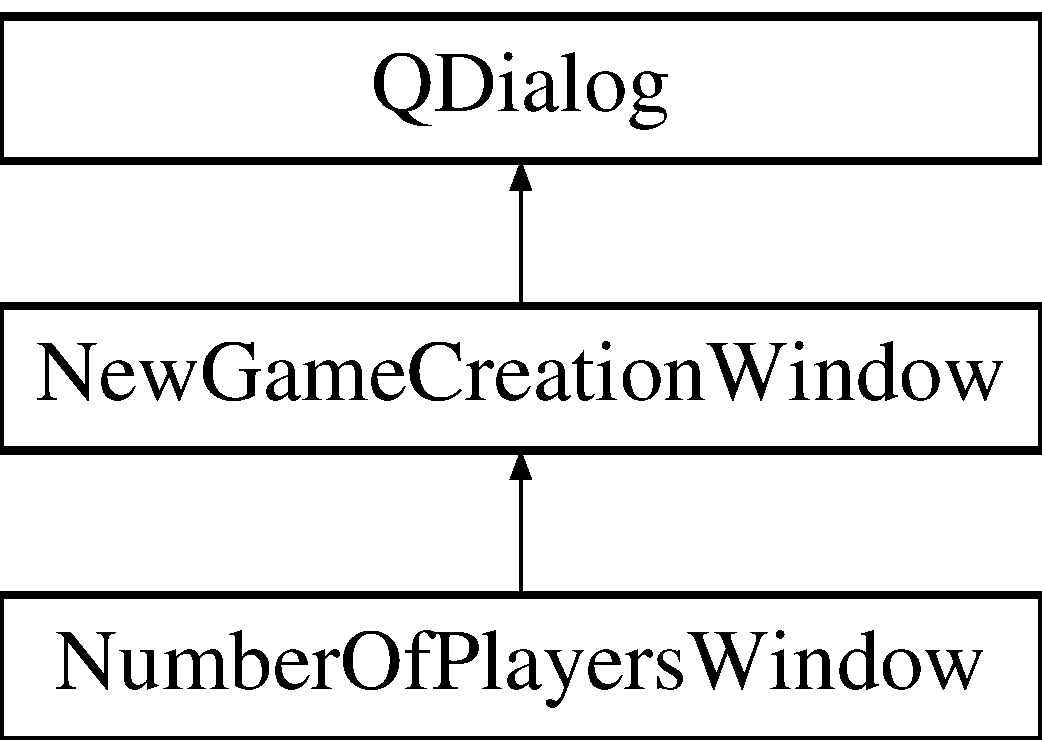
\includegraphics[height=2.000000cm]{classNumberOfPlayersWindow}
\end{center}
\end{figure}
\subsection*{Public Member Functions}
\begin{DoxyCompactItemize}
\item 
\mbox{\Hypertarget{classNumberOfPlayersWindow_a522ce7de553a78ef1514cc988abb8d38}\label{classNumberOfPlayersWindow_a522ce7de553a78ef1514cc988abb8d38}} 
{\bfseries Number\+Of\+Players\+Window} (\hyperlink{classNewGameCreator}{New\+Game\+Creator} $\ast$\hyperlink{classNumberOfPlayersWindow_a7a4c90e2553e4f401fde3ec81e7e3f56}{new\+Game\+Creator}, Q\+Widget $\ast$parent=0)
\end{DoxyCompactItemize}
\subsection*{Private Slots}
\begin{DoxyCompactItemize}
\item 
void \hyperlink{classNumberOfPlayersWindow_a7fe10b716af29b5cca42267a391587ec}{enable\+Confirm\+Button} ()
\begin{DoxyCompactList}\small\item\em Enable the confirm button. \end{DoxyCompactList}\item 
void \hyperlink{classNumberOfPlayersWindow_aaebac1245ca92099446f0cac82304dab}{confirm\+Button\+Clicked} ()
\begin{DoxyCompactList}\small\item\em Function called when the confirm button of the window is clicked. \end{DoxyCompactList}\end{DoxyCompactItemize}
\subsection*{Private Member Functions}
\begin{DoxyCompactItemize}
\item 
void \hyperlink{classNumberOfPlayersWindow_afefa90be1b7ddf10ac84744a7b79816d}{close\+Event} (Q\+Close\+Event $\ast$e)
\begin{DoxyCompactList}\small\item\em Reimplementation of Q\+Dialog\+::close\+Event() \end{DoxyCompactList}\end{DoxyCompactItemize}
\subsection*{Private Attributes}
\begin{DoxyCompactItemize}
\item 
\mbox{\Hypertarget{classNumberOfPlayersWindow_a56a9fa50a2568bd693ec4ac0b1c4c2a4}\label{classNumberOfPlayersWindow_a56a9fa50a2568bd693ec4ac0b1c4c2a4}} 
Q\+Push\+Button $\ast$ \hyperlink{classNumberOfPlayersWindow_a56a9fa50a2568bd693ec4ac0b1c4c2a4}{confirm\+Button}
\begin{DoxyCompactList}\small\item\em The confirm button of the window. \end{DoxyCompactList}\item 
\mbox{\Hypertarget{classNumberOfPlayersWindow_a2faa8f67709fa2da57936c57236be6c7}\label{classNumberOfPlayersWindow_a2faa8f67709fa2da57936c57236be6c7}} 
Q\+Radio\+Button $\ast$ \hyperlink{classNumberOfPlayersWindow_a2faa8f67709fa2da57936c57236be6c7}{number\+Of\+Players\+Radio\+Button} \mbox{[}M\+A\+X\+\_\+\+N\+U\+M\+B\+E\+R\+\_\+\+O\+F\+\_\+\+P\+L\+A\+Y\+E\+RS -\/ M\+I\+N\+\_\+\+N\+U\+M\+B\+E\+R\+\_\+\+O\+F\+\_\+\+P\+L\+A\+Y\+E\+RS+1\mbox{]}
\begin{DoxyCompactList}\small\item\em Array to keep the pointers to the radio buttons in the window. \end{DoxyCompactList}\item 
\mbox{\Hypertarget{classNumberOfPlayersWindow_a7a4c90e2553e4f401fde3ec81e7e3f56}\label{classNumberOfPlayersWindow_a7a4c90e2553e4f401fde3ec81e7e3f56}} 
\hyperlink{classNewGameCreator}{New\+Game\+Creator} $\ast$ \hyperlink{classNumberOfPlayersWindow_a7a4c90e2553e4f401fde3ec81e7e3f56}{new\+Game\+Creator}
\begin{DoxyCompactList}\small\item\em Pointer to the \hyperlink{classNewGameCreator}{New\+Game\+Creator} instance. \end{DoxyCompactList}\end{DoxyCompactItemize}


\subsection{Detailed Description}
Window used to insert the number of players in the game. 

The valid numbers of players are shown to the user by means of radio buttons, and he can select the correct number. 

\subsection{Member Function Documentation}
\mbox{\Hypertarget{classNumberOfPlayersWindow_afefa90be1b7ddf10ac84744a7b79816d}\label{classNumberOfPlayersWindow_afefa90be1b7ddf10ac84744a7b79816d}} 
\index{Number\+Of\+Players\+Window@{Number\+Of\+Players\+Window}!close\+Event@{close\+Event}}
\index{close\+Event@{close\+Event}!Number\+Of\+Players\+Window@{Number\+Of\+Players\+Window}}
\subsubsection{\texorpdfstring{close\+Event()}{closeEvent()}}
{\footnotesize\ttfamily void Number\+Of\+Players\+Window\+::close\+Event (\begin{DoxyParamCaption}\item[{Q\+Close\+Event $\ast$}]{e }\end{DoxyParamCaption})\hspace{0.3cm}{\ttfamily [private]}}



Reimplementation of Q\+Dialog\+::close\+Event() 


\begin{DoxyParams}{Parameters}
{\em e} & The Q\+Close\+Event instance\\
\hline
\end{DoxyParams}
To avoid that the window is closed by the user not in the proper way (i.\+e., by pressing the confirm button), this function is reimplemented. In particular, when a close event is created, it is ignored by the window and so the window doesn\textquotesingle{}t close. \mbox{\Hypertarget{classNumberOfPlayersWindow_aaebac1245ca92099446f0cac82304dab}\label{classNumberOfPlayersWindow_aaebac1245ca92099446f0cac82304dab}} 
\index{Number\+Of\+Players\+Window@{Number\+Of\+Players\+Window}!confirm\+Button\+Clicked@{confirm\+Button\+Clicked}}
\index{confirm\+Button\+Clicked@{confirm\+Button\+Clicked}!Number\+Of\+Players\+Window@{Number\+Of\+Players\+Window}}
\subsubsection{\texorpdfstring{confirm\+Button\+Clicked}{confirmButtonClicked}}
{\footnotesize\ttfamily void Number\+Of\+Players\+Window\+::confirm\+Button\+Clicked (\begin{DoxyParamCaption}{ }\end{DoxyParamCaption})\hspace{0.3cm}{\ttfamily [private]}, {\ttfamily [slot]}}



Function called when the confirm button of the window is clicked. 

When the confirm button of the window is clicked, this function detects which radio button was selected by the user in order to discover the number of players in the game, which is passed to the \hyperlink{classGame}{Game} class, and then signals to \hyperlink{classMainWindow}{Main\+Window} that the next window for data insertion must be shown. \mbox{\Hypertarget{classNumberOfPlayersWindow_a7fe10b716af29b5cca42267a391587ec}\label{classNumberOfPlayersWindow_a7fe10b716af29b5cca42267a391587ec}} 
\index{Number\+Of\+Players\+Window@{Number\+Of\+Players\+Window}!enable\+Confirm\+Button@{enable\+Confirm\+Button}}
\index{enable\+Confirm\+Button@{enable\+Confirm\+Button}!Number\+Of\+Players\+Window@{Number\+Of\+Players\+Window}}
\subsubsection{\texorpdfstring{enable\+Confirm\+Button}{enableConfirmButton}}
{\footnotesize\ttfamily void Number\+Of\+Players\+Window\+::enable\+Confirm\+Button (\begin{DoxyParamCaption}{ }\end{DoxyParamCaption})\hspace{0.3cm}{\ttfamily [private]}, {\ttfamily [slot]}}



Enable the confirm button. 

By default, the confirm button of the window is disabled, since when the window is shown no radio button is checked, which means that the number of players is at that moment not selected. When one of these radio buttons is checked by the user, this radio button calls activate\+Confirm\+Button() to enable the confirm button of the window to allow the user to click it and confirm the selected number of players. 

The documentation for this class was generated from the following files\+:\begin{DoxyCompactItemize}
\item 
gui/Number\+Of\+Players\+Window.\+h\item 
gui/Number\+Of\+Players\+Window.\+cpp\end{DoxyCompactItemize}

\hypertarget{classPlayer}{}\section{Player Class Reference}
\label{classPlayer}\index{Player@{Player}}
\subsection*{Private Attributes}
\begin{DoxyCompactItemize}
\item 
\mbox{\Hypertarget{classPlayer_af9c920fabaafdeb7961a645315b521ff}\label{classPlayer_af9c920fabaafdeb7961a645315b521ff}} 
std\+::string {\bfseries name}
\item 
\mbox{\Hypertarget{classPlayer_a331c99cd2b2686a1c45344e57ee8d0b2}\label{classPlayer_a331c99cd2b2686a1c45344e57ee8d0b2}} 
int {\bfseries number\+Of\+Cards}
\item 
\mbox{\Hypertarget{classPlayer_a0d69dcd849a3085041015c0a99389f1a}\label{classPlayer_a0d69dcd849a3085041015c0a99389f1a}} 
int {\bfseries weapon\+Card\+Set}
\item 
\mbox{\Hypertarget{classPlayer_a4006d4bab3208cf3243c8364d48e2667}\label{classPlayer_a4006d4bab3208cf3243c8364d48e2667}} 
int {\bfseries suspect\+Card} \mbox{[}9\mbox{]}
\item 
\mbox{\Hypertarget{classPlayer_af9b61df991a2f7fed88feabad6737d8e}\label{classPlayer_af9b61df991a2f7fed88feabad6737d8e}} 
int {\bfseries room\+Card} \mbox{[}9\mbox{]}
\end{DoxyCompactItemize}


The documentation for this class was generated from the following files\+:\begin{DoxyCompactItemize}
\item 
game/Player.\+h\item 
game/Player.\+cpp\end{DoxyCompactItemize}

\hypertarget{classReasoner}{}\section{Reasoner Class Reference}
\label{classReasoner}\index{Reasoner@{Reasoner}}


The documentation for this class was generated from the following files\+:\begin{DoxyCompactItemize}
\item 
reasoner/Reasoner.\+h\item 
reasoner/Reasoner.\+cpp\end{DoxyCompactItemize}

\hypertarget{classRecapWindow}{}\section{Recap\+Window Class Reference}
\label{classRecapWindow}\index{Recap\+Window@{Recap\+Window}}
Inheritance diagram for Recap\+Window\+:\begin{figure}[H]
\begin{center}
\leavevmode
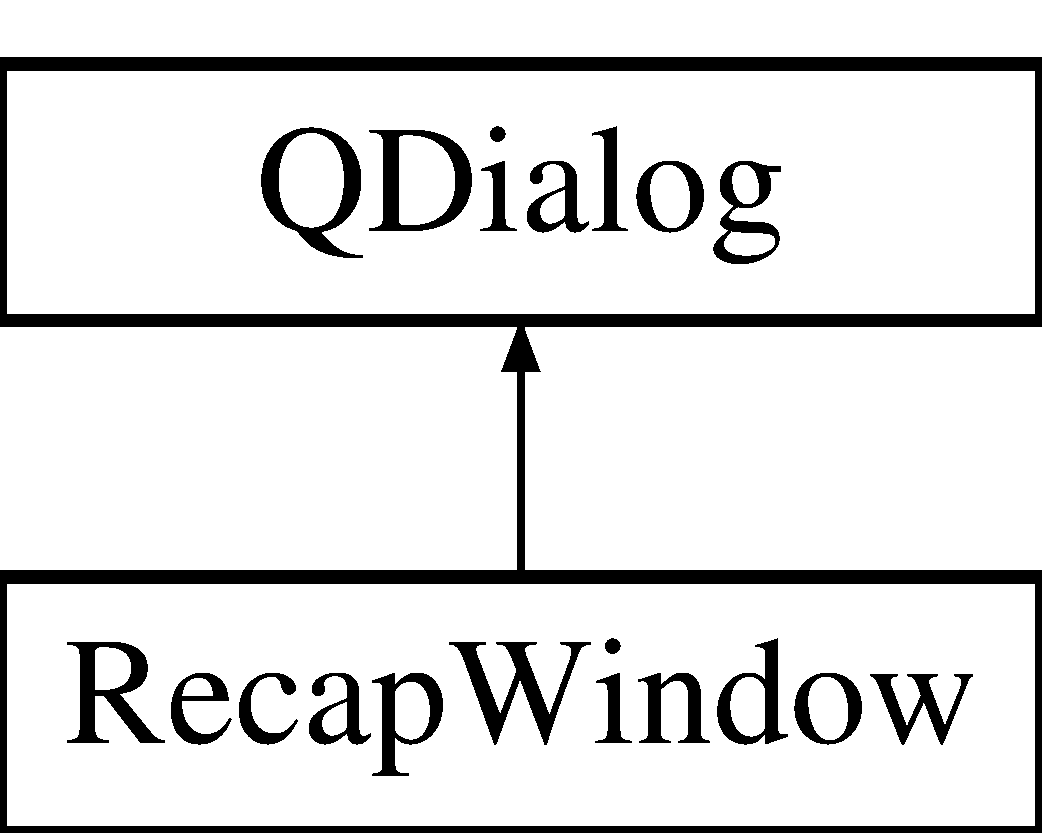
\includegraphics[height=2.000000cm]{classRecapWindow}
\end{center}
\end{figure}
\subsection*{Public Member Functions}
\begin{DoxyCompactItemize}
\item 
\mbox{\Hypertarget{classRecapWindow_a0f89f24533eeeb2c5d91376dc14c5602}\label{classRecapWindow_a0f89f24533eeeb2c5d91376dc14c5602}} 
{\bfseries Recap\+Window} (\hyperlink{classNewGameCreator}{New\+Game\+Creator} $\ast$new\+Game\+Creator, Q\+Widget $\ast$parent=0)
\end{DoxyCompactItemize}
\subsection*{Private Slots}
\begin{DoxyCompactItemize}
\item 
\mbox{\Hypertarget{classRecapWindow_ae285e915c54b2c7c7315cc9e1d671397}\label{classRecapWindow_ae285e915c54b2c7c7315cc9e1d671397}} 
void {\bfseries open\+Next\+Window} ()
\end{DoxyCompactItemize}
\subsection*{Private Attributes}
\begin{DoxyCompactItemize}
\item 
\mbox{\Hypertarget{classRecapWindow_a46bcf1b62d62dd9cfa6e20a78f7f60f0}\label{classRecapWindow_a46bcf1b62d62dd9cfa6e20a78f7f60f0}} 
\hyperlink{classNewGameCreator}{New\+Game\+Creator} $\ast$ {\bfseries new\+Game\+Creator}
\end{DoxyCompactItemize}


The documentation for this class was generated from the following files\+:\begin{DoxyCompactItemize}
\item 
gui/Recap\+Window.\+h\item 
gui/Recap\+Window.\+cpp\end{DoxyCompactItemize}

%--- End generated contents ---

% Index
\backmatter
\newpage
\phantomsection
\clearemptydoublepage
\addcontentsline{toc}{chapter}{Index}
\printindex

\end{document}
